\documentclass[12pt, a4paper]{article}

\usepackage[utf8]{inputenc}
\usepackage[framemethod=TikZ]{mdframed}
\usepackage[hidelinks]{hyperref}
\usepackage{mathtools, amssymb, amsmath, cleveref, fancyhdr, geometry, graphicx, float, subfigure, arydshln, url, setspace, framed, pifont, physics, ntheorem, tcolorbox, utopia}
%%% for coding %%%
\usepackage{listings}
\usepackage[ruled, vlined, linesnumbered]{algorithm2e}

\geometry{a4paper, left=2cm, right=2cm, bottom=2cm, top=2cm}

\pagestyle{fancy}
\fancyhead{}
\fancyhead[L]{\leftmark}
\fancyhead[R]{\rightmark}
\fancyfoot{}
\fancyfoot[C]{\thepage}
%\renewcommand{\headrulewidth}{0pt}
\renewcommand{\footrulewidth}{0pt}

\hypersetup{
	colorlinks = true,
	bookmarks = true,
	bookmarksnumbered = true,
	pdfborder = 001,
	linkcolor = blue
}

\definecolor{grey}{rgb}{0.49,0.38,0.29}
\definecolor{mygreen}{rgb}{0,0.6,0}


%%% for coding %%%
\lstset{basicstyle = \ttfamily\small,commentstyle = \color{mygreen}\textit, deletekeywords = {...}, escapeinside = {\%*}{*)}, frame = single, framesep = 0.5em, keywordstyle = \bfseries\color{blue}, morekeywords = {*}, emph = {self}, emphstyle=\bfseries\color{red}, numbers = left, numbersep = 1.5em, numberstyle = \ttfamily\small\color{grey},  rulecolor = \color{black}, showstringspaces = false, stringstyle = \ttfamily\color{purple}, tabsize = 4, columns = flexible}

\newcounter{index}[subsection]
\setcounter{index}{0}
\newenvironment*{df}[1]{\par\noindent\textbf{Definition \thesubsection.\stepcounter{index}\theindex\ (#1).}}{\par}

\newenvironment*{eg}[1]{\begin{framed}\par\noindent\textbf{Example \thesubsection.\stepcounter{index}\theindex\ #1} \par}{\par\end{framed}}

\newenvironment*{thm}[1]{\begin{tcolorbox}\par\noindent\textbf{Theorem \thesubsection.\stepcounter{index}\theindex\ #1} \par}{\par\end{tcolorbox}}

\newenvironment*{cor}[1]{\par\noindent\textbf{Corollary \thesubsection.\stepcounter{index}\theindex\ #1}}{\par}
\newenvironment*{lem}[1]{\par\noindent\textbf{Lemma \thesubsection.\stepcounter{index}\theindex\ #1}}{\par}
\newenvironment*{ax}[1]{\par\noindent\textbf{Axiom \thesubsection.\stepcounter{index}\theindex\ #1}}{\par}
\newenvironment*{prop}[1]{\par\noindent\textbf{Proposition \thesubsection.\stepcounter{index}\theindex\ #1}}{\par}
\newenvironment*{conj}[1]{\par\noindent\textbf{Conjecture \thesubsection.\stepcounter{index}\theindex\ #1}}{\par}
\newenvironment*{nota}{\par\noindent\textbf{Notation \thesubsection.\stepcounter{index}\theindex.}}{\par}


\newcounter{nprf}[subsection]
\setcounter{nprf}{0}
\newenvironment*{prf}{\par\indent\textbf{\textit{Proof \stepcounter{nprf}\thenprf.}}}{\hfill$\blacksquare$\par}
\newenvironment*{dis}{\par\indent\textbf{\textit{Disproof \stepcounter{nprf}\thenprf.}}}{\hfill$\blacksquare$\par}
\newenvironment*{sol}{\par\indent\textbf{\textit{Solution \stepcounter{nprf}\thenprf.}}\par}{\hfill{$\square$}\par}

\newtheorem{hint}{Hint.}[section]
\newtheorem{rmk}{Remark.}[section]
\newtheorem{ext}{Extension.}[section]
\newtheorem{clm}{Claim.}[section]

\linespread{1.25}

\title{\textbf{Emory University\\\textbf{MATH 315 Numerical Analysis}\\ Learning Notes}}
\author{Jiuru Lyu}
\date{\today}

\def\Z{{\mathbb{Z}}}
\def\R{{\mathbb{R}}}
\def\C{{\mathbb{C}}}
\def\Q{{\mathbb{Q}}}
\def\E{{\mathbb{E}}}
\def\d{{\mathrm{d}}}
\def\float{\texttt{float}}
\def\flt{\texttt{float}}
\def\Inf{\texttt{Inf}}
\def\NaN{\texttt{NaN}}
\def\epsilon{\varepsilon}
\def\emptyset{\varemptyset}
\def\A{\vb A}
\def\dsst{\displaystyle}
\def\bigO{\mathcal{O}}
\def\pqed{\quad\square}
\def\st{\emph{\ s.t.\ }}
\def\hat{\widehat}
\def\tilde{\widetilde}
\def\l{\ell}

\begin{document}
\maketitle

\tableofcontents

\newpage
\section{Floating Point Numbers}
\subsection{Binary Representation}
\begin{df}{Binary}
	$0$ and $1$; on and off.	
\end{df}
\begin{eg}{Represent Numbers in Base-2}
	\par Consider $13=1(10)+3(1)=1(10)+3(10^0)$ in base-10. It can be converted into base-2 by decomposing $13$ as $1(2^3)+1(2^2)+0(2^1)+1(2^0)$.
\end{eg}
\begin{eg}{Fractions in Base-2}
	\[\dfrac{7}{16}=\dfrac{1}{16}(7)=\qty(2^{-4})\qty(2^2+2^1+2^0)=2^{-2}+2^{-3}+2^{-4}.\]
\end{eg}
\begin{eg}{Repeating Fractions in Base-2}
	\[\begin{aligned}\dfrac{1}{5}=\dfrac{1}{8}+\epsilon_1\quad&\Longrightarrow\quad\epsilon_1=\dfrac{1}{5}-\dfrac{1}{8}=\dfrac{8-5}{(5\times8)}=\dfrac{3}{40}\\\epsilon_1=\dfrac{3}{3(16)}+\epsilon_2\quad&\Longrightarrow\quad\cdots\end{aligned}\] Repeating the steps above, we would finally get \[\dfrac{1}{5}=\dfrac{1}{8}+\dfrac{1}{16}+\dfrac{1}{128}+\dfrac{1}{256}+\cdots\]
\end{eg}
\begin{thm}{}
	Let $n\in\Z$ and $n\geq1$, then \[\sum_{k=0}^{n-1}2^k=2^{n-1}+2^{n-2}+\cdots+2^0=2^n-1.\]	
\end{thm}
\subsection{Integers in Computers}
\begin{df}{Storing Integers}
	\texttt{unit8} stands for unsigned integers and \texttt{int8} stands for signed integers. 
	\begin{rmk} The $8$ here represents $8$ bits. It is a measure of how much storage (how many $0$s or $1$s).\end{rmk}
	\[\begin{aligned}
	\begin{tabular}{|c|c|c|c|c|c|c|c|}
		\hline
		\ $b_7$&$b_6$\ &\ $b_5$&$b_4$\ &\ $b_3$&$b_2$\ &\ $b_1$&\ $b_0$\\
		\hline
	\end{tabular}&\\
	\begin{tabular}{ccccccccc}	
		unsigned: &$2^7$&$2^6$&$2^5$&$2^4$&$2^3$&$2^2$&$2^1$&$2^0$\\
		signed:   &$-2^7$&$2^6$&$2^5$&$2^4$&$2^3$&$2^2$&$2^1$&$2^0$
	\end{tabular}&
	\end{aligned}\]
\end{df}
\begin{eg}{}
	\[\texttt{unit8}(13)=00001101\] Since $-13=1(-2^7)+1(2^6)+1(2^5)+1(2^4)+0(2^3)+0(2^2)+1(2^1)+1(2^0)$, we have \[\texttt{int8}(-13)=11110011\]
\end{eg}
\begin{rmk}
	Largest and Smallest Integers: \[\begin{aligned}\textnormal{\texttt{uint8}}(x_L)&=11111111\quad\Longrightarrow x_L=2^7+2^6+\cdots+2^0=2^8-1=255\\\textnormal{\texttt{uint8}}(x_S)&=00000000\quad\Longrightarrow x_S=0(2^7)+0(2^6)+\cdots+0(2^0)=0\\\textnormal{\texttt{int8}}(x_L)&=01111111\quad\Longrightarrow x_L=0(-2^7)+2^6+\cdots+2^0=2^7-1=127\\\textnormal{\texttt{int8}}(x_S)&=100000000\quad\Longrightarrow x_S=1(-2^7)+0(2^6)+\cdots+0(2^0)=-128\end{aligned}\]	
\end{rmk}
\subsection{Representation of Floating Point Numbers}
\begin{df}{Normalized Scientific Notation}
	Only $1$ digit (non-zero) to the left of the decimal point.	
\end{df}
\begin{eg}{}
	\[\begin{aligned}123.456\times10^7&\\12.3456\times10^8&\\1.23456\times10^9&\rightarrow\text{normalized}\end{aligned}\]	
\end{eg}
\begin{df}{Anatomy of Floating Point Numbers}
	A floating point number, $\texttt{float}(x)$, consists of three parts: $s(x)$ (sign bit), $e(x)$ (exponent bits), and $f(x)$ (fraction bits).
\end{df}
\begin{df}{Precision}
	Precision is defined by the number 	of bits per part:
	\begin{center}\begin{tabular}{c|c|c|c|c}
	&$s(x)$&$e(x)$&$f(x)$&total\\\hline
	double precision (DP)&$1$&$11$&$52$&$64$\\
	single precision (SP)&$1$&$8$&$23$&$32$\\
	half precision (HP)&$1$&$5$&$10$&$16$\\
	\end{tabular}\end{center}
	\begin{rmk}The less bits the float point number has, the less storage it requires and faster computation it performs, but more error introduces.\end{rmk}
\end{df}
\begin{df}{Floating Point Number}
	\begin{equation}\label{eq1}\texttt{float}(x)=(-1)^{s(x)}\qty(1+\dfrac{f(x)}{2^\text{\# of fraction bits}})2^{E(x)},\end{equation} where $E(x)$ is called the \textit{unbiased exponent} because it is centered about $0$ and is calculated through the $e(x)$, the \textit{biased exponent} because it can only be non-negative integers, by the following formula: \[E(x)=e(x)-\qty(2^{\text{\# of exponent bits}-1}-1).\]	
	\begin{rmk}
		Eq. (\ref{eq1}) is in normalized scientific notation because the largest number $f(x)$ can represent is $2^\textnormal{\# of fraction bits}-1$. Hence, \[1+\dfrac{f(x)}{2^\textnormal{\# of fraction bits}}<2,\] and thus there will be only $1$ digit in front of the decimal point.
	\end{rmk}
\end{df}
\begin{eg}{Formula for a Floating Point Number in Double Precision (DP)}
	\[\texttt{float}_\text{DP}(x)=(-1)^{s(x)}\qty(1+\dfrac{f(x)}{2^{52}})2^{e(x)-1023}.\]	
\end{eg}
\begin{eg}{Converting DP into Decimal}
	\par Suppose a DP floating number is stored as $s(x)=0$, $e(x)=10000000011,$ and $f(x)=0100100\cdots0$. Find its representation in decimal base-10.
	\begin{sol}
		$e(x)=10000000011=2^{10}+2^{1}+2^{0}$ and $f(x)=0100100\cdots0=2^{50}+2^{47}$. Then, the unbiased exponent $E(x)=e(x)-1023=2^{10}+2^1+2^0-\qty(2^{10}-1)=4$. So, \[\begin{aligned}\texttt{float}_\text{DP}(x)&=(-1)^{s(x)}+\qty(1+\dfrac{f(x)}{2^{52}})2^{E(x)}\\&=(-1)^0\qty(1+\dfrac{2^{50}+2^{47}}{2^{52}})2^4\\&=\qty(1+2^{-2}+2^{-5})2^4\\&=2^4+2^2+2^{-1}\\&=16+4+0.5=20.5\end{aligned}\]
	\end{sol}
\end{eg}
\begin{eg}{Converting Value to DP}
	\par Suppose a number in base-10 is $-10.75$. Find its representation of floating point number under DP.
	\begin{sol}
	We have
		\[\begin{aligned}\texttt{value}(x)=-10.75&=(-1)(10+0.75)\\&=(-1)\qty(2^3+2^1+2^{-1}+2^{-2})\\&=(-1)\qty(1+2^{-2}+2^{-4}+2^{-5})2^3\quad\qty\Big[\text{In normalized scientific notation}]\\&=(-1)^1\qty(1+\dfrac{2^{50}+2^{48}+2^{47}}{2^{52}})2^{1026-1023}\\&=(-1)^1\qty(1+\dfrac{2^{50}+2^{48}+2^{47}}{2^{52}})2^{2^{10}+2^{1}-1023}\end{aligned}\]So, we have $s(x)=1$, $e(X)=10000000010$, and $f(x)=010110\cdots0$.
	\end{sol}
\end{eg}
\begin{thm}{Some Special Rules}
	\begin{enumerate}
		\item The formula \[\texttt{value}(x)=(-1)^{s(x)}+\qty(1+\dfrac{f(x)}{2^{52}})2^{e(x)-1023}\] only holds when $0<e(x)<2^{11}-1$ or $00\cdots01<e(x)<11\cdots10$.
		\item If $e(x)=11\cdots1$, then it encodes special numbers.
		\item If $e(x)=00\cdots0$: 
		\begin{itemize}
			\item If $f(x)=00\cdots0$, then $\texttt{value}(x)=0$.
			\item If $f(x)>0$, it encodes a \textit{denormalized floating point number}: \[\texttt{value}(x)=(-1)^{s(x)}\qty(0+\dfrac{f(x)}{2^{52}})2^{-1022}.\] This denormalized floating point number is more precise when describing really small things. 
		\end{itemize}
	\end{enumerate}
\end{thm}
\begin{df}{Machine Epsilon/$\epsilon_\text{WP}$}
	Let ``WP'' stands for the working precision (DP/SP/HP/etc.). The \textit{machine epsilon}, denoted as $\epsilon_\text{WP}$, is the gap between $1$ and the next largest floating point number. Equivalently, it can be viewed as the smallest possible non-zero value of $\dfrac{f(x)}{2^\text{number of fraction bits}}$. So, $\epsilon_\text{DP}=2^{-52}$, $\epsilon_\text{SP}=2^{-23}$, and $\epsilon_\text{HP}=2^{-10}$.
\end{df}
\begin{df}{Special Numbers}
	\begin{enumerate}
		\item $\pm0$: when $s(x)=\pm1$ and $e(x)=f(x)=0$.
		\item $\pm\Inf$
		\item $\NaN$: not-a-number
	\end{enumerate}	
\end{df}
\begin{df}{Floating Point Arithmetic}
	\begin{enumerate}
		\item The set of real numbers, $\R$, is closed under arithmetic operations.
		\item The set of all WP floating point numbers, however, is not closed under arithmetic operations. For example, $\texttt{float}_\text{DP}(x)=\texttt{float}_\text{DP}(y)=2^{52}+1$, but $xy=2^{104}+\epsilon$ cannot be represented using DP. 
		\item Suppose $x$ and $y$ are floating point numbers, then $x\oplus y=\texttt{float}(x+y)$ and $x\otimes y=\texttt{float}(xy)$. Consider \texttt{float} as a rounding process, we can also define subtraction and division of floating point numbers. 
	\end{enumerate}	
\end{df}
\begin{eg}{}
	Assume we are only allowed three significant digits (in Base-10) in a computer. Suppose $x=1.23\times10^4$ and $y=6.54\times10^3$. Find $x\oplus y=\texttt{float}(x+y)$.
	\begin{sol}
		\[\begin{aligned}x\oplus y&=\texttt{float}(x+y)\\&=\texttt{float}(1.23\times10^4+6.54\times10^3)\\&=\texttt{float}(1.23\times10^4+0.654\times10^3)\\&=\texttt{float}(1.884\times10^4)\\&=1.88\times10^4.\end{aligned}\]
	\end{sol}
\end{eg}

\subsection{Errors}
\begin{df}{Errors We May See}
	\begin{enumerate}
		\item \textit{Overflow}: The exponent is too large. This means $\qty|x|$ is large and the computer will represent it as $\pm\Inf.$ Note: In DP, $x_\text{large}=\qty(2-2^{-52})\times2^{1023}\approx1.798\times10^{308}$. This number is referred as \texttt{realmax} in MATLAB.
		\item \textit{Underflow}: Large negative exponent. This means $\qty|x|$ is tiny and the computer will represent it as $\pm0$. Note: In SP, $x_\text{small}\approx2.225\times10^{-53}$ and is referred as \texttt{realmin} in MATLAB.
		\item \textit{Roundoff error}: cutoff or round at some point. 
	\end{enumerate}	
	Note that sometimes we are encounter the catastrophic cancellation, meaning the subtraction leads to our loss of significance or information. In this case, it is different from underflow error or roundoff error.
\end{df}
\begin{eg}{Catastrophic Cancellation/Loss of Significance Due to Subtraction}
	\[\begin{aligned}x&=3.141592920353983\approx\dfrac{355}{113}&\quad16\text{ digits}\\y&=3.141592653589794\approx\pi&\quad16\text{ digits}\\x-y&=0.000000266764189&\quad9\text{ digits}\end{aligned}\]
\end{eg}
\begin{df}{Relative Error}
	Let $z\in\R$. The relative error between $\float(z)$ and $z$ is denoted as $\mu$ and \[\mu=\dfrac{\float(z)-z}{z}\]\[\float(z)=z(1+\mu),\] where we know \[\qty|\mu|\leq\dfrac{\epsilon_\text{WP}}{2}.\]
\end{df}
\begin{eg}{Propagation of Errors}
	There are two major sources of errors: storing number and arithmetics. \par Consider a computer only allow $3$ significant figures. Then $\epsilon_\text{WP}=0.01$.\par Consider $x=\dfrac{1}{3}$, $y=\dfrac{8}{7}$, and $x+y=\dfrac{31}{21}$. Then, \[\float(x)=0.333=3.33\times10^{-1}=x\qty(1+\mu_x).\] Solving for $\mu_x$: \[\begin{aligned}\dfrac{333}{1000}&=\dfrac{1}{3}\qty(1+\mu_x)\\\mu_x&=\dfrac{999}{1000}-1=\dfrac{-1}{1000}=-0.001\end{aligned}\] Note that $\qty|\mu_x|=0.01<\dfrac{\epsilon_\text{WP}}{2}$. Similarly, we can solve  $\float(y)=1.14\times10^0=y\qty(1+\mu_y)$ for $\qty|\mu_y|=0.0025$. Now, consider the floating point addition \[\begin{aligned}x\oplus y&=\flt(\flt(x)+\flt(y))\\&=\flt(3.33\times10^{-1}+1.14\times10^0)\\&=\flt(1.473\times10^0)\\&=1.47\times10^0.\end{aligned}\] Also, solve $x\oplus y=(x+y)\qty(1+\mu_a)$ for $\qty|\mu_a|=0.0042$. Note that \[\qty|\mu_x|+\qty|\mu_y|=0.0035<0.0042=\qty|\mu_a|.\] This is called the propagation of error. 
\end{eg}
\begin{eg}{Plotting Exponentials Using Factored and Expanded Forms}
	Consider $p(x)=(1-x)^{10}$ and its expanded form.
	Plot them to see which is better. 
	\begin{lstlisting}[language = Matlab, title = {Example 1.4.5}]
	%% Defining the Functions
	p_1 = @(x) (1-x).^10;
	p_2 = @(x) x.^10-10*x.^9+45*x.^8-120*x.^7+210*x.^6-252*x.^5+...
			210*x.^4-120*x.^3+45*x.^2-10*x+1;
	%% Ploting the Functions
	x = linspace(0, 2, 100);
	plot(x, p_1(x))
	hold on
	plot(x, p_2(x))
	legend("Factor", "Expanded")
	%% Zooming In
	y = linspace(0.99, 1.01, 100);
	hold off
	plot(y, p_1(y))
	hold on
	plot(y, p_2(y))
	legend("Factor", "Expanded")
	\end{lstlisting}
	\begin{figure}[H]\centering
	\subfigure[Plotting Functions]{\label{plottingFuc}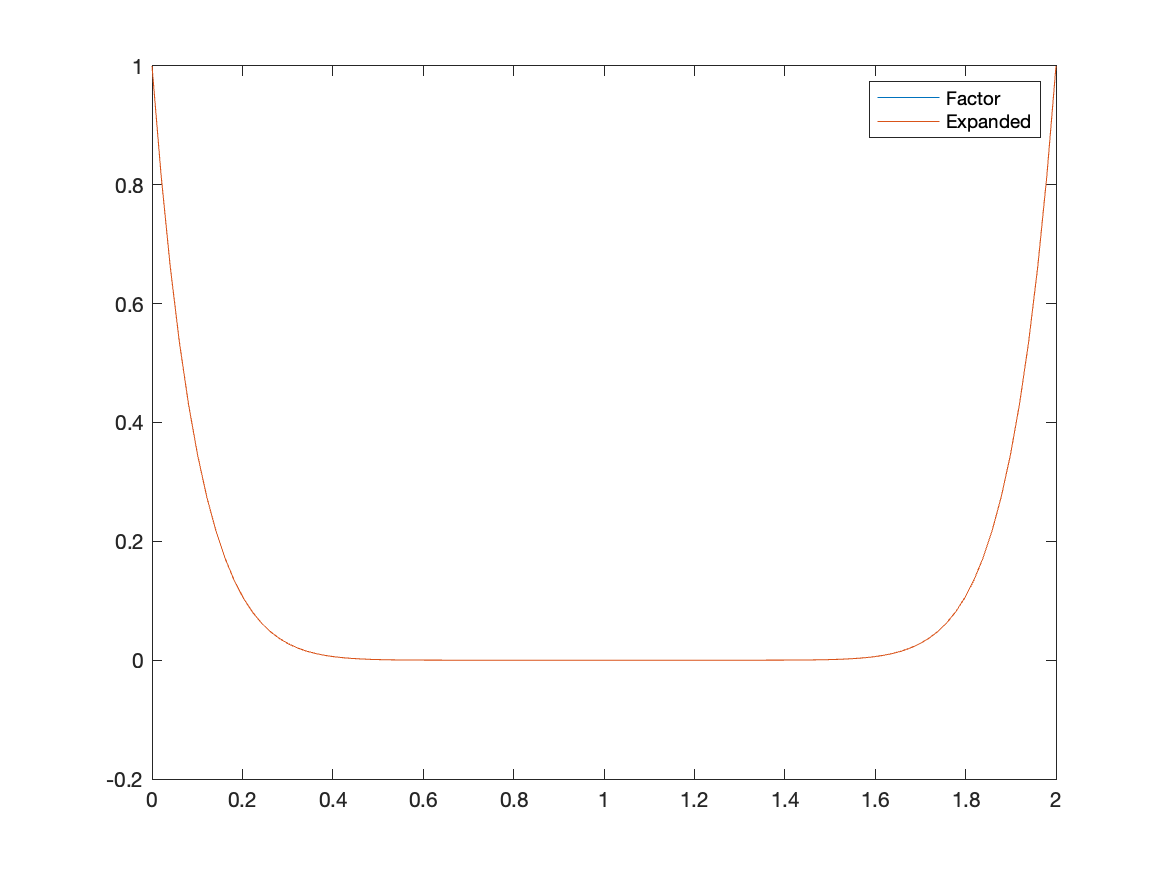
\includegraphics[width=0.48\textwidth]{figs/Ex2_3_1_Ploting_Functions}}
	\hfill
	\subfigure[Zooming In]{\label{zoomingIn}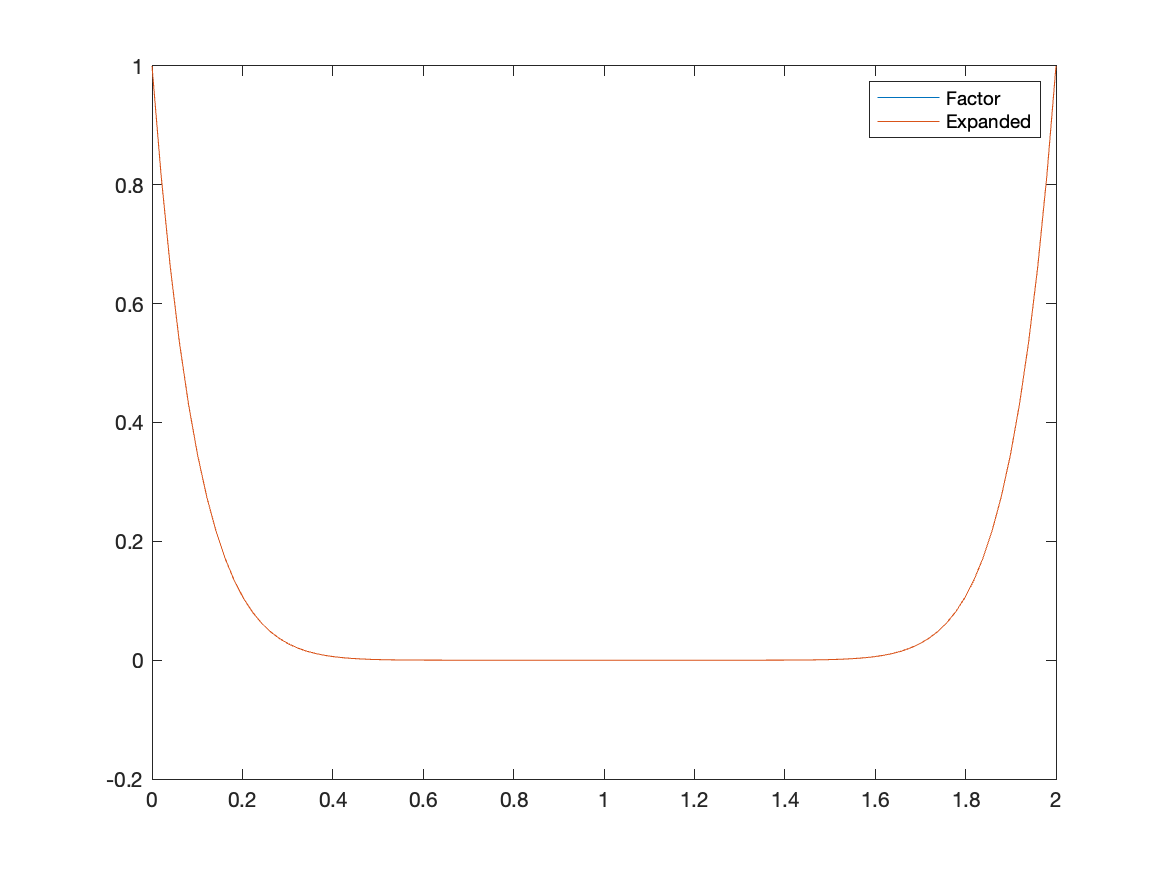
\includegraphics[width=0.5\textwidth]{figs/Ex2_3_1_Ploting_Functions}}\end{figure}
	It seems that the two functions are the same (Fig \ref{plottingFuc}); however if we zooming in (Fig \ref{zoomingIn}), the expanded version introduces more error than the factored version because the expanded version requires more arithmetical operations in it. 
	\end{eg}

\newpage
\section{Solutions of Linear Systems}
\begin{rmk} Assumption throughout this chapter: $\A$ is a square $n\times n$ matrix. \end{rmk}
\subsection{Simply Solved Linear Systems}
\begin{df}{Linear System}
	\begin{itemize}
		\item Equation form: $x_i$ are variables (what we solve for) and $a_{ij}$ are coefficients: \begin{align*}a_{11}x_1+a_{12}x_2+\cdots+a_{1n}x_n&=b_1\\a_{21}x_1+a_{22}x_2+\cdots+a_{2n}x_n&=b_2\\\vdots\\a_{n1}x_1+a_{n2}x_2+\cdots+a_{nn}x_n&=b_n\end{align*} This system has $n$ equations and $n$ variables. 
		\item Matrix form: \[\mqty[a_{11}&a_{12}&\cdots&a_{1n}\\a_{21}&a_{22}&\cdots&a_{2n}\\\vdots&\vdots&\ddots&\vdots\\a_{n1}&a_{n2}&\cdots&a_{nn}]\mqty[x_1\\x_2\\\vdots\\x_n]=\mqty[b_1\\b_2\\\vdots\\b_n]\implies \A x=b,\] where $\A$ is the coefficient matrix, a $n\times n$ matrix, $x$ is the unknown, the solution vector with length $n$, and $b$ is the right hand side, vector with length $n$.
	\end{itemize}	
\end{df}
\begin{thm}{Number of Solutions to a Linear System}
	A linear system $\A x=b$ could have the following numbers of solutions: 
	\begin{itemize}
		\item One unique solution: $\A x=b$ is nonsingular; $\A$ is invertible.
		\item No solutions: $\A x=b$ is singular.
		\item Infinite many solutions: $\A x=b$ is singular. 
	\end{itemize}	
\end{thm}
\begin{thm}{Matrix-Vector Multiplication}
	Let $\A\in\R^{m\times n}$ and $x\in\R^n$. 
	\begin{itemize}
		\item View 1: Row-wise. Let $y=\A x$, then $\dsst y_i=\sum_{j=1}^n a_{ij}x_j$ as the $i^\text{th}$ row of $y$. 
		\item View 2: Column-wise. $\A x$ is a linear combination of columns of $\A$. So, $\dsst y=\sum_{j=1}^nx_j\va{a_j}$, where we regard $\A$ as $\mqty[\va{a_1}&\va{a_2}&\cdots&\va{a_n}]$
	\end{itemize}	
\end{thm}
\begin{lstlisting}[language = Matlab, title = {Row-Wise Vector Multiplication}]
y = zeros(n, 1);
for i = 1:n % loop over rows
	for j = 1:n % loop over sum
		y(i) = y(i) + A(i,j) + x(j);
	end
end
\end{lstlisting}
\begin{lstlisting}[language = Matlab, title = {Row-Wise Vector Multiplication (Vectorization)}]
y = zeros(n, 1);
for i = 1:n % loop over rows
	y(i) = A(i,:) * x(i); % vectorization
end
\end{lstlisting}
\begin{lstlisting}[language = Matlab, title = {Column-Wise Vector Multiplication}]
y = zeros(n, 1);
for j = 1:n % loop over columns
	y = y + x(j) * A(:, j);
end
\end{lstlisting}
\begin{df}{Important Part of a Matrix}
	\begin{itemize}
		\item Diagonal Part
		\item Strictly Upper Triangular Part
		\item Strictly Lower Triangular Part
	\end{itemize}	
\end{df}
\begin{thm}{Solving Diagonal Matrix}
	Given \[\mqty[a_{11}&&\\&\ddots&\\&&a_{nn}]\mqty[x_1\\\vdots\\x_n]=\mqty[b_1\\\vdots\\b_n],\] we have \[a_{11}x_1=b_1;\quad a_{22}x_2=b_2;\quad\cdots\quad a_{nn}x_n=b_n\] So we have \[x_i=\dfrac{b_i}{a_{ii}},\] only if $a_{ii}\neq0.$
	\begin{rmk}$a_{ii}\neq0$ holes if $\A$ is invertible. \end{rmk}
\end{thm}
\begin{rmk}A Diagonal matrix is also a lower triangular matrix or an upper triangular matrix. \end{rmk}
\begin{lstlisting}[language = Matlab, title = {Solving Diagonal Matrix}]
x = zeros(n, 1);
for i = 1:n
	x(i) = b(i) / A(i,i); % overflow and underflow
end
\end{lstlisting}
\begin{thm}{Solving Lower Triangular Systems}
	Given \[\mqty[a_{11}&&&\\a_{21}&a_{22}&&\\\vdots&&\ddots&\\a_{n1}&\cdots&&a_{nn}]\mqty[x_2\\x_2\\\vdots\\x_n]=\mqty[b_1\\b_2\\\vdots\\v_n],\] we have \begin{align*}a_{11}x_1&=b_1\\a_{21}x_1+a_{22}x_{2}&=b_2\\\vdots\\a_{n1}x_1+a_{n2}x_2+\cdots+a_{nn}x_n&=b_n\end{align*} We can use the Forward Substitution to solve: \[x_i=\dfrac{b_1-a_{i1}x_1-a_{i2}x_2-\cdots-a_{i(i-1)}x_{i-1}}{a_{ii}.}\]
\end{thm}
\begin{algorithm}\caption{Row-Oriented Forward Substitution}\SetKwData{And}{\rmfamily{\textbf{and}}}\SetKwData{Or}{\rmfamily{\textbf{or}}}\SetKwData{Break}{\rmfamily{\textbf{break}}}
\KwIn{matrix $\A=\mqty[a_{ij}]$; vector $b=\mqty[b_i]$}
\KwOut{solution vector $x=\mqty[x_i]$}
\BlankLine\Begin{
	\For(\tcp{loop over rows}){i = 1 \KwTo n} { 
		\For(\tcp{loop over columns}) {j = 1 \KwTo i-1} {
			$b_i \coloneqq b_i-a_{ij}x_j$\;
		}
		$x_i \coloneqq b_i/a_{ii}$\;
	}
}
\end{algorithm}
\begin{eg}{}
	Given \[\mqty[-5&&\\3&3&\\2&-5&3]\mqty[x_1\\x_2\\x_3]=\mqty[-10\\3\\21].\] Use column-wise forward substitution to solve this system. 
	\begin{sol}
		In column-wise: \[x_1\mqty[-5\\3\\2]+x_2\mqty[0\\3\\-5]+x_3\mqty[0\\0\\4]=\mqty[-10\\3\\21].\]	
		\begin{enumerate}
			\item Step 1: Solve for $x_1=-10/-5=2.$
			\item Step 2: Plug $x_1=2$ into the equation: \[x_2\mqty[0\\3\\-5]+x_3\mqty[0\\0\\4]=\mqty[-10\\3\\21]-(2)\mqty[-5\\3\\2]=\mqty[0\\-3\\17].\]
			\item Step 3: Solve for $x_2=-3/3=-1$.
			\item Step 4: Plug $x_2=-1$ into the equation: \[x_3\mqty[0\\0\\4]=\mqty[0\\-3\\17]-(-1)\mqty[0\\3\\-5]=\mqty[0\\0\\12].\]
			\item Step 5: Solve for $x_3=12/4=3.$
		\end{enumerate}
	\end{sol}
\end{eg}
\begin{algorithm}\caption{Column-Oriented Forward Substitution}\SetKwData{And}{\rmfamily{\textbf{and}}}\SetKwData{Or}{\rmfamily{\textbf{or}}}\SetKwData{Break}{\rmfamily{\textbf{break}}}
\KwIn{matrix $\A=\mqty[a_{ij}]$; vector $b=\mqty[b_i]$}
\KwOut{solution vector $x=\mqty[x_i]$}
\BlankLine\Begin{
	\For{j = 1 \KwTo n} { 
		$x_j\coloneqq b_j/a_{jj}$\;
		\For{i = j+1 \KwTo n} {
			$b_i \coloneqq b_i-a_{ij}x_j$\;
		}
	}
}
\end{algorithm}
\begin{thm}{Computational Cost of Forward Substitution}
	Number of floating point operations ($+$, $-$, $\times$, $/$) in row $i$ is $1$ division, $(i-1)$ multiplications, and $(i-1)$ subtractions. So, Number of floating points operations, or flops, of the algorithm is \begin{align*}\text{flops}=\sum_{i=1}^n(1+i-1+i-1)&=\sum_{i=1}^n(2i-1)\\&=2\sum_{i=1}^ni-\sum_{i=1}^n1\\&=2\qty[\dfrac{(n+1)(n)}{2}]-n\\&=n^2\end{align*}
	\begin{rmk}It should be the same number of flops if we do column-oriented forward substitution. \end{rmk}
	\begin{rmk} Solving upper triangular system using backward substitution. \end{rmk}
\end{thm}

\subsection{GEPP and Matrix Factorization}
\begin{thm}{Gaussian Elimination}
	In Gaussian Elimination, we are allowed to 
	\begin{enumerate}
		\item Swap rows (exchange, pivot)
		\item Add multiple of one row to another
		\item Multiply row by non-zero scalar. 
	\end{enumerate}
\end{thm}
\begin{rmk}We require the equation with the largest coefficient in magnitude at the top when doing the Gaussian Elimination. This is because we want to divide by large numbers instead of smaller ones (which will cause errors).\end{rmk}
\begin{algorithm}\caption{General Structure of GEPP}\SetKwData{And}{\rmfamily{\textbf{and}}}\SetKwData{Or}{\rmfamily{\textbf{or}}}\SetKwData{Break}{\rmfamily{\textbf{break}}}

\BlankLine\Begin{
	\For{\text{all stages}} { 
		\text{pivot}\;
		\text{eliminate}\;
	}
}
\end{algorithm}
\begin{lstlisting}[language = Matlab, title = {At stage $k$, eliminate $x_k$, from rows $k+1$ to $n$}]
for i = k+1:n
	m(i,k) = a(i,k) / a(k,k); % find the multiplier
	a(i,k) = 0;
	for j = k+1:n
		a(i,j) = a(i,j) - m(i,k) * a(k,j); % could use vectorization
	end
	b(i) = b(i) - m(i,k) * b(k);
end
\end{lstlisting}
\begin{lstlisting}[language = Matlab, title = {Pivoting at stage $k$: find the coefficient with the largest magnitude}]
%% The code tells us which row has the pivot.
p = k;
for i = k+1:n
	if abs(a(p,k)) < abs(a(i,k))
		p = i;
	end
end
%% Swap rows in A and b
A([p,k],:) = A([k,p],:);
b(p) = b(k);
\end{lstlisting}
\begin{thm}{Cost of GEPP}
	At stage $k$, we only focus on rows $k$ through $n$ and columns $k$ through $n$. We have $(n-k)$ divisions for multipliers. For every multiplier we have $(n-k)$ multiplications, which are then used $(n-k)$ times to change each row. So, we have $(n-k)(n-k)$ multiplications in total. Subtractions come with multiplications, so we also have $(n-k)(n-k)$ subtractions. 
\end{thm}
\begin{thm}{Another Perspective on GEPP}
	The process of GEPP can be written as matrix multiplication $\vb E\vb A$, where $\vb E$ is an elementary matrix and act on the rows of $\vb A$.	
\end{thm}
\begin{thm}{Matrix Factorizations: $\vb P\vb A=\vb L\vb U$}
	\[\vb P\vb A=\vb L\vb U,\] where $\vb U$ is upper-triangular, $\vb L$ is lower-triangular, and $\vb P$ is the pivot or permutation matrix.\par 
	This factorization comes from GEPP. Almost all matrices $\vb A$ have $\vb P\vb A=\vb L\vb U$ unless we have a column of all zeros in $\vb A$. \par
\end{thm}
\begin{thm}{Solving $\vb Ax=b$ with $\vb P\vb A=\vb L\vb U$}
	Given $\vb Ax+b$ and pre-computed $\vb P\vb A=\vb L\vb U$: \begin{align*}\vb P\vb A&=\vb Pb\\\vb L\vb U&=\vb Pb\\\vb Ux&=\vb L^{-1}\vb Pb&\text{using forward substitution}\\x&=\vb U^{-1}\vb L^{-1}\vb Pb&\text{using backward substitution}\end{align*}
	This process need around $\bigO\qty(n^2)$ operations. $\bigO(\cdot)$ is the big-O notation, meaning the number is dominated by $n^2$.
\begin{lstlisting}[language=Matlab, title={$\vb P\vb A=\vb L\vb U$ in MATLAB}]
[L, U, P] = lu(A);
% P could be omitted sometimes. 
\end{lstlisting}
\end{thm}
\begin{thm}{Cholesky Factorization}
	If $\A$ is symmetric ($\A=\A^T$) and positive definite (all eigenvalues are positive), then $\A=\vb R^T\vb R$, where $\vb R$ is upper-triangular and $\vb R^T$ is lower-triangular. This factorization is $2$ time less expensive than GEPP. 
\end{thm}
\begin{rmk}
	Choleksy Factorization is just the $\vb P\A=\vb L\vb U$ factorization for SPDs (symmetric positive definite matrices).
\end{rmk}
\begin{thm}{Other Matrix Factorization}
\begin{enumerate}
	\item $\vb Q\vb R$ decomposition: \[\A=\vb Q\vb R,\] where $\vb R$ is upper-triangular and $\vb Q$ is orthogonal such that $\vb Q^T\vb Q=\vb Q^T\vb Q=\vb I$.\par  $\vb Q$ is really easy to be inverted and comes from the Gram-Schmidt process. \par This composition is a bit more expensive than $\vb P\A=\vb L\vb U$.
	\item Singular Value Decomposition (SVD): \[\vb A=\vb U\vb\Sigma\vb V^T,\] where $\vb U$ and $\vb V^T$ are orthogonal and $\vb\Sigma$ is diagonal. This factorization is also more expensive than $\vb P\A=\vb L\vb U$ decomposition.
\end{enumerate}
\end{thm}

\subsection{Measuring Accuracy of Solutions}
\begin{df}{Vector Norms}
	A vector norm is a function $\|\cdot\|:\R^n\to\R$ that satisfies
	\begin{itemize}
		\item \textbf{Positive Definiteness}: $\|x\|\geq0\quad\forall x\in\R^n$ and $\|x\|=0$ if and only if $x=0$.
		\item \textbf{Positive Homogeneity}: $\|cx\|=\qty|c|\|x\|\quad\forall x\in\R^n$ and $c\in\R$.
		\item \textbf{Triangular Inequality}: $\|x+y\|\leq\|x\|+\|y\|\quad\forall x,y\in\R^n$.
	\end{itemize}	
\end{df}
\begin{df}{Common Definitions of Norm}
	\begin{itemize}
		\item Pythagorean Distance: $\|x\|_2=\sqrt{x_1^2+x_2^2+\cdots+x_n^2}$.
		\item Taxicab/Manhattan Distance: $\|x\|_1=\qty|x_1|+\qty|x_2|+\cdots+\qty|x_n|$.
		\item Infinity Norm: $\|x\|_\infty=\dsst\max_{i=1,\dots,n}\qty|x_i|$.
	\end{itemize}	
\end{df}
\begin{prf}
	In this prove, we want to show the $1-$norm is a proper norm.
	\begin{itemize}
		\item \textbf{Positive Definiteness}: Note that $\|x\|_1=\qty|x_1++\cdots+\qty|x_n|\geq0$ since each $\qty|x_j|\geq0$. If one $x_i\neq0$, $\qty|x_i|\geq0$, then $\|x\|_1>0$. So, if $\|x\|_1=0$, it must be $x=0$. $\pqed$
		\item \textbf{Positive Homogeneity}: \begin{align*}\|cx\|_1&=\qty|cx_1|+\qty|cx_2|+\cdots+\qty|cx_n|\\&=\qty|c|\qty|x_1|+\qty|c|\qty|x_2|+\cdots+\qty|c|\qty|x_n|\\&=\qty|c|\qty(\qty|x_1|+\qty|x_2|+\cdots+\qty|x_n|)\\&=\qty|c|\|x\|_1.\pqed\end{align*}
		\item \textbf{Triangle Inequality}: \begin{align*}\|x+y\|_1&=\qty|x_1+y_1|+\qty|x_2+y_2|+\cdots+\qty|x_n+y_n|\\&\leq\qty|x_1|+\qty|y_1|+\qty|x_2|+\qty|y_2|+\cdots+\qty|x_n|+\qty|y_n|\\&=\qty(\qty|x_1|+\qty|x_2|+\cdots+\qty|x_n|)+\qty(\qty|y_1|+\qty|y_2|+\cdots+\qty|y_n|)\\&=\|x\|_1+\|y\|_1.\end{align*}
	\end{itemize}	
\end{prf}
\begin{df}{Matrix Norm}
	A matrix norm is a function $\|\cdot\|:\R^{n\times n}\to\R\st$
	\begin{itemize}
		\item \textbf{Positive Definiteness}: $\|\A\|\geq0$ and $\|\A\|=0$ if and only if $\A=0$.
		\item \textbf{Positive Homogeneity}: $\|c\A\|=\qty|c|\|\A\|$.
		\item \textbf{Triangle Inequality}: $\|\A+\vb{B}\|\leq\|\A\|+\|\vb{B}\|$.
	\end{itemize}	
\end{df}
\begin{df}{Some Matrix Norms}
	\begin{enumerate}
		\item \textbf{Frobenius Norm}: \[\|\A\|_F=\sqrt{\sum_{j=1}^n\sum_{i=1}^na_{ij}^2}.\]
		\item \textbf{Induced Matrix Norm}: Let $\A\in\R^{n\times n}$, $x\in\R^{n\times1}$, and $p=1,2,\infty,\cdots$, then \[\|\A\|_p=\max_{x\neq0}\dfrac{\|\A x\|_p}{\|x\|_p}=\max_{\|x\|_p=1}\|\A x\|_p.\]
	\end{enumerate}	
\end{df}
\begin{rmk}Induced norm intuition: how much does $\|x\|_p$ change when we apply $\A$?\end{rmk}
\begin{thm}{Induced Matrix Norms with different $p$'s}
	\begin{itemize}
		\item $\|\A\|_2=\sigma_1$, the largest singular value. That is, if $\A=\vb U\vb\Sigma\vb V^T$, then $\|\A\|_2$ is the largest entry in $\vb\Sigma$.
		\item $\dsst\|\A\|_1=\max_{j=1,\dots,n}\sum_{i=1}^n\qty|a_{ij}|$, the maximum column sum.
		\item $\dsst\|\A\|_\infty=\max_{i=1,\dots,n}\sum_{j=1}^n\qty|a_{ij}|$, the maximum row sum. 
	\end{itemize}	
\end{thm}
\begin{prf}
	Let's show that $\|\A\|_1$ is the maximum column sum. We will (1) show $\|\A\|_1\leq$ the maximum column sum, and (2) find one case when we attain the upper bound. Given $\|x\|_1=1$, then \begin{align*}\|\A x\|_1=\sum_{i=1}^n\qty|\underbrace{\sum_{j=1}^n a_{ij}x_{j}}_{i-\text{th entry of}\A x}|&\leq\sum_{i=1}^n\sum_{j=1}^n\qty|a_{ij}|\qty|x_j|\\&=\sum_{j=1}^n\qty|x_j|\qty(\sum_{i=1}^n\qty|a_{ij}|)\\&\leq\max_{j=1,\dots,n}\sum_{i=1}^n\qty|a_{ij}|,\text{ when }x\text{ has exactly 1}\text{ entry equal to }1.\end{align*} When $x=e_{j^*}$ be a standard basis vector with $1$ in $j^*$ position, where $j^*$ is the column of $\A$ with maximum column sum, we have \[\|\A e_{j^*}\|_1=\|j-\text{th column of }\A\|_1=\max_{j=1,\dots,n}\sum_{i=1}^n\qty|a_{ij}|.\]	
\end{prf}
\begin{eg}{}
	Given that $\A=\mqty[-1&2\\-12&9]$, find $\|\A\|_1$ and $\|\A\|_\infty$.
	\[\|\A\|_1=\text{maximum column sum}=\max_{j=1,\dots,n}\|\A(:.j)\|_1=13.\]
	\[\|\A\|_\infty=\text{maximum row sum}=21.\]
\end{eg}
\begin{thm}{Submultiplicativity of Induced Norm}
	\[\|\A x\|_p\leq\|\A\|_p\|x\|_p.\]
\end{thm}
\begin{prf}
	By definition, we know $\dsst\|\A\|_p=\max_{x\neq0}\dfrac{\|\A x\|_p}{\|x\|_p}$. Then, \begin{align*}\|\A\|_p&\geq\dfrac{\|\A x\|_p}{\|x\|_p}\\\|\A x\|_p&\leq\|\A\|_p\|x\|_p.\end{align*}	
\end{prf}
\begin{cor}{}
	$\|\A\vb B\|_p\leq\|\A\|_p\|\vb B\|_p.$	
\end{cor}
\begin{df}{Measuring Erros}
	Suppose $x$ is the true solution, and $\hat{x}$ is the approximate solution. Then \begin{align*}\textit{Error}&=\|\hat{x}-x\|\\\textit{Relative Error}&=\dfrac{\|\hat{x}-x\|}{\|x\|},\quad x\neq0.\end{align*}	
	\begin{rmk}In practice, we do not know $x$, the true solution. So this measurement cannot be used.\end{rmk}
\end{df}
\begin{df}{Residual}
	We know $\vb A$, $b$, $\hat{x}$, and we want to solve $\vb Ax=b$. So, the \begin{align*}\textit{Residual}&=\A\hat{x}-b\\\textit{Residual Norm}&=\|\A\hat{x}-b\|\\\textit{Relative Residual Norm}&=\dfrac{\|\A\hat{x}-b\|}{\|b\|}\end{align*}
	
\end{df}
\begin{eg}{}
	Let $\A=\mqty[0.835&0.667\\0.333&0.266], b=\mqty[0.168\\0.067].$ Let $x=\mqty[1\\-1]$ be the exact solution to the system $\A x=b$ and $\hat{x}=\mqty[267\\-334]$, a bad computation of the solution. Then, \begin{align*}\dfrac{\|b-\A\hat{x}\|_2}{\|x\|_2}&\approx0.006\\\dfrac{\|x-\hat{x}\|_2}{\|x\|_2}&\approx\bigO(10^2)\end{align*}	
	\begin{rmk}	The residual norm is not always a good estimate of the relative error.\end{rmk}
\end{eg}
\begin{df}{Ill-Conditioned, Well-Conditioned}
	If the system is linearly dependent, we call the system \textit{ill-conditioned}. If the system is linearly independent, we call it \textit{well-conditioned}.	
\end{df}
\begin{df}{Condition Numbers}
	The condition number of $\A$ is $\kappa\qty(\A)=\|\A\|\|\A^{-1}\|$. Note that $\kappa(\A)\geq1$ and $\kappa(\vb I)=1$. If $\kappa(\A)$ is large, then $\A$ is ill-conditioned. If $\kappa(\A)$ is close to $1$, then $\A$ is well-conditioned. 	
\end{df}
\begin{rmk}
	Some intuition on $\kappa(\A)$: 
	\begin{itemize}
		\item $\|\A\|$: how much $\A$ moves $x$: $\A x=b$.
		\item $\|\A^{-1}\|$: how much $\A^{-1}$ moves $b$: $x=\A^{-1}b$.
	\end{itemize}
	So, if $\kappa(\A)=\|\A\|\|\A^{-1}\|$ is close to $1$, the moves balance each other. If $\kappa(\A)$ is large, then we move the vectors a lot. 
\end{rmk}
\begin{thm}{Upper Bound for Relative Error}
	\[\underbrace{\dfrac{\|x-\hat{x}\|}{\|x\|}}_\text{Relative Error}\leq\kappa(\A)\cdot\underbrace{\dfrac{\|b-\A\hat{x}\|}{\|b\|}}_\text{Relative Residual}=\|\A\|\|\A^{-1}\|\dfrac{\|b-\A\hat{x}\|}{\|b\|}.\]	
\end{thm}
\begin{prf}
	We want to use residual norm to compare $\|x-\hat{x}\|$ and $\|x\|$. Suppose $x$ is the true solution: $b=\A x$. Then, \[\|b\|=\|\A x\|\leq\|\A\|\|x\|.\] So, \begin{equation}\label{eq2}\dfrac{1}{\|x\|}\leq\dfrac{\|\A\|}{\|b\|}\end{equation} Consider the residual: $r=b-\A\hat{x}=\A x-\A\hat{x}=\A\qty(x-\hat{x}).$ So, $x-\hat{x}=\A^{-1}r$. Therefore, \begin{equation}\label{eq3}\|x-\hat{x}\|=\|\A^{-1}r\|\leq\|\A^{-1}\|\|r\|\end{equation} Putting Eq. (\ref{eq2}) and Eq. (\ref{eq3}) together, we have \[\|x-\hat{x}\|\cdot\dfrac{1}{\|x\|}\leq\|\A^{-1}\|\|r\|\cdot\dfrac{\|\A\|}{\|b\|}\] Re-arrange the inequality, we have \[\dfrac{\|x-\hat{x}\|}{\|x\|}\leq\|\A\|\|\A^{-1}\|\dfrac{\|b-\A\hat{x}\|}{\|b\|}.\]
\end{prf}
\begin{rmk}
	Since norms measure how far two things are apart from each other, $\|x-\hat{x}\|=\|\hat{x}-x\|$ and $\|b-\A\hat{x}\|=\|\A\hat{x}-b\|$.
\end{rmk}
\begin{cor}{}
	If $\kappa(\A)\approx1$, then a small residual implies that $\hat{x}$ is a good approximation to the true solution $x$. If $\kappa(\A)$ is large, then we still don't know if $\hat{x}$ is a good approximation to the true solution. 
\end{cor}
\begin{eg}{}
	Given $\A_1=\mqty[1&10\\0&1]$ and $\A_2=\mqty[1&10^6\\0&1]$. Which matrix will have a better approximation to the true solution? 
	\begin{sol}
		\[\kappa_1(\A_1)=\|\A_1\|_1\|\A^{-1}_1\|_1.\] Since $\det(\A_1)=1-0=1,$ we know $\A_1^{-1}=\dfrac{1}{\det(\A_1)}\mqty[1&-10\\0&1]=\mqty[1&-10\\0&1].$ So, \[\kappa_1(\A_1)=\|\A_1\|_1\|\A^{-1}_1\|_1=(11)(11)=121.\] Similarly, \[\kappa_2(\A_2)=\|\A_2\|_1\|\A_2^{-1}\|_1=\qty(1+10^6)\qty(1+10^6)=\bigO(10^12).\] Since $\kappa_2(\A_2)\gg\kappa_1(\A_1)$, $\A_1$ will yield a more accurate approximation.
	\end{sol}
	\begin{rmk}
		Think $\kappa(\A)$ as an indicator for how much movement of $x$ will there be if we apply $\A$ on $x$.	
	\end{rmk}
\end{eg}
\begin{clm}
	Conditioning is inherent to the problem. So, no algorithms can improve conditioning.
\end{clm}
\begin{df}{Algorithm Stability/Backward Stability}
	When we solve $\A x=b$, we will have some algorithm $\hat{x}=\text{algorithm}(\A,b)$. Imagine we run the algorithm in reverse (backwards). We should obtain $\hat{\A}$ and $\hat{b}\st\hat{\A}\hat{x}=\hat{b}$ in exact arithmetic. An algorithm is \textit{backward stable} if $\|\A-\hat{\A}\|$ and $\|b-\hat{b}\|$ are small.	
\end{df}
\begin{rmk}
	Algorithm stability has nothing to do with conditioning.	
\end{rmk}
\begin{eg}{}
	Given $\A=\mqty[\alpha&1\\1&2]$. We know that solving $\A x=b$ using Gaussian Elimination without pivoting, we could get a solution far from true. So, Gaussian Elimination without pivoting is not backward stable. In contrast, GEPP is a backward stable algorithm. 
\end{eg}
\begin{eg}{Is Multiplication Backward Stable?}
	Define \[x\otimes y=\float(\float(x)\times\float(y))\] on a computer with $3$ significant digits. Suppose $x=\dfrac{1}{3}$ and $y=\dfrac{1}{2}$. Then, \[x\otimes y=\float((0.333)(0.500)=0.167;\quad\epsilon_\text{WP}=1.01-1.00=10^{-2}\] Take $\hat{x}=0.334$ and $\hat{y}=0.500$, we get $\hat{x}\hat{y}=0.167$. Since $\|x-\hat{x}\|\approx0.001\leq\dfrac{1}{2}\epsilon_\text{WP}$, we say multiplication is backward stable. Similarly, we could show all floating point operations are backward stable, in fact. 
\end{eg}
\begin{eg}{}
	Prove that $\|\vb Qx\|_2=\|x\|_2$ for any $x\in\R^{n}$ if $\vb Q$ is orthogonal. 
	\begin{prf}
		Since $\vb Q$ is orthogonal, $\vb Q^T\vb Q=\vb Q\vb Q^T=\vb I$. Note that the $2-$norm: \[\|x\|_2^2=x_1^2+x_2^2+\cdots+x_n^2=x^Tx.\] Then, \[\|\vb Qx\|_2^2=\qty(\vb Qx)^T\qty(\vb Qx)=x^T\vb Q^T\vb Qx=x^Tx=\|x\|_2^2.\] So, \[\|\vb Qx\|_2=\|x\|_2.\]
	\end{prf}
	\begin{ext} What is $\|\vb Q\|_2$? What is $\kappa(\vb Q)$?	\end{ext}
	\begin{sol}
		\[\|\vb Q\|_2=\max_{\|x\|_2=1}\dfrac{\|\vb Qx\|_2}{\|x\|_2}=\max_{\|x\|_2=1}\dfrac{\|x\|_2}{\|x\|_2}=\max_{\|x\|_2=1}1=1.\]
		\[\kappa(\vb Q)=\|\vb Q\|_2\|\vb Q^{-1}\|_2=\|\vb Q\|_2\|\vb Q^T\|_2=1\cdot1=1.\]
	\end{sol}
\end{eg}

\newpage
\section{Curve Fitting}
\subsection{Polynomial Interpolation}
\begin{df}{Interpolation}
	A function $p(x)$ interpolates data $\qty{\qty(x_i, f_i)}_{i=0}^N$ if $p(x_i)=f_i$ for $i=0,\dots,N$.
\end{df}
\begin{rmk} Uniqueness of the interpolating polynomial. \end{rmk}
\begin{df}{Polynomial}
	A polynomial $p_k(x)$ is of \textit{degree} $k$ if there are constants $c_0,\dots,c_k\st$\[p_k(x)=c_0+c_1x+\cdots+c_kx^k.\] A polynomial $p_k(x)$ is in \textit{exact degree} $k$ if $c_k\neq0$.
\end{df}
\begin{thm}{Steps for Polynomial Interpolation}
	\begin{enumerate}
		\item Create a problem.
		\begin{itemize}
			\item Find some data.
			\item Design the problem
		\end{itemize}
		\item Choose a degree (based on the number of interpolation points)
		\item Determine the coefficients. $\rightarrow$ Construct a polynomial
		\begin{itemize}
			\item Choose a polynomial basis
			\item Solve a linear system.
		\end{itemize}
		\item Draw the curve: evaluating at lots of points. $\rightarrow$ Evaluate a polynomial
	\end{enumerate}	
\end{thm}
\begin{algorithm}\caption{Constructing a Polynomial Interpolant}
\SetKwData{And}{\rmfamily{\textbf{and}}}\SetKwData{Or}{\rmfamily{\textbf{or}}}\SetKwData{Break}{\rmfamily{\textbf{break}}}
\KwIn{data, $\qty{\qty(x_i, f_i)}_{i=0}^N$; polynomial basis: $\qty{q_j(x)}_{i=0}^N$}
\KwOut{$c_0,\dots,c_M\st\dsst\sum_{j=0}^Mc_jq_j(x_i)=f_i$ for $i=0,\dots,N$}
	Solve for $c_0,\dots,c_M$: \[\begin{cases}c_0q_0(x_0)+c_1q_1(x_0)+\cdots+c_Mq_M(x_0)=f_0\\\vdots\\c_0q_0(x_N)+c_1q_1(x_N)+\cdots+c_Mq_M(x_N)=f_0\end{cases}\] \[\mqty[q_0(x_0)&\cdots&q_M(x_0)\\\vdots&\ddots&\vdots\\q_0(x_N)&\cdots&q_M(x_N)]\mqty[c_1\\\vdots\\c_M]=\mqty[f_0\\\vdots\\f_N]\]
\end{algorithm}
\begin{thm}{Polynomial Uniqueness}
	When the nodes $\qty{\qty(x_i, f_i)}_{i=0}^N$ are distinct, there is a unique polynomial, the interpolating polynomial $p_N(x)$ of degree $N$ that interpolates the data. That is,  \[\mqty[q_0(x_0)&\cdots&q_M(x_0)\\\vdots&\ddots&\vdots\\q_0(x_N)&\cdots&q_M(x_N)]\in\R^{n\times n}\]
\end{thm}
\begin{df}{Power Series}
	\[p_N(x)=c_0+c_1x+c_2x^2+\cdots+c_Nx^N\]
	The Vandermonde Matrix is defined as \[\mqty[1&x_0&\cdots&x_0^N\\\vdots&\vdots&\ddots&\vdots\\1&x_N&\cdots&x_N^N].\]
	\begin{itemize}
		\item Pros: easy to understand and implement
		\item Cons: ill-conditioning, near singularity of the Vandermonde matrix, when $\qty|x_i-x_j|$ is small. 
	\end{itemize}
\end{df}
\begin{eg}{Power Series}
	Interpolate the points $\qty{(-1,0), (0,1), (1,3)}$.
	\begin{sol}
		Suppose $p_2(x)=c_0+c_1x+c_2x^2$. Then, \begin{align*}(-1,0):\ p_2(-1)&=c_0+c_1(-1)+c_2(-1)^2=0\\(0,1):\ p_2(0)&=c_0+c_1(0)+c_2(0^2)=1\\(1,3):\ p_2(1)&=c_0+c_1(1)+c_2(1)^2=3.\end{align*} In matrix form: \[\mqty[1&-1&1\\1&0&0\\1&1&1]\mqty[c_0\\c_1\\c_2]=\mqty[0\\1\\3]\implies\mqty[c_0\\c_1\\c_2]=\mqty[1\\3/2\\1/2].\]
	\end{sol}
\end{eg}
\begin{df}{Newton Form}
	\[p_N(x)=b_0+b_1\qty(x-x_0)+b_2(x-x_0)(x-x_1)+\cdots+b_N(x-x_0)(x-x_1)\cdots(x-x_{N-1}).\]
	\begin{itemize}
		\item Pros: we are having a lower triangular system: 
		\begin{align*}p_N(x_0)&=b_0\\p_N(x_1)&=b_0+b_1(x-x_0)\\p_N(x_2)&=b_0+b_1(x-x_0)+b_2(x-x_0)(x-x_1).\end{align*}
	\end{itemize}
\end{df}
\begin{eg}{Newton Form}
	Interpolate the points $\qty{(-1,0), (0,1), (1,3)}$.
	\begin{sol}
		\begin{align*}p_N(x)&=b_0+b_1(x-(-1))+b_2(x-(-1))(x-0)\\p_N(-1)&=b_0\\p_N(0)&=b_0+b_1\\p_N(1)&=b_1+2b_1+2b_2\end{align*} In matrix form: \[\mqty[1&0&0\\1&1&0\\1&2&2]\mqty[b_0\\b_1\\b_2]=\mqty[0\\1\\3]\xrightarrow[\text{Substitution}]{\text{Forward}}\mqty[b_0\\b_1\\b_2]=\mqty[0\\1\\1/2].\]
	\end{sol}
\end{eg}
\begin{df}{Lagrange Polynomials}
	\begin{itemize}
		\item Coefficient $=$ function values $f_i$. $\Longrightarrow$ we don't need to solve anything
		\item \[\l(x):\begin{cases}1\quad\text{at }x=x_i\\0\quad\text{ at}x=x_j,\ j\neq i\end{cases}\] Now, we want to construct a polynomial that has roots at all the nodes: \[\omega(x)=(x-x_0)(x-x_1)\cdots(x-x_N).\] Then, if we assume we have distinct noes, we have \[\l_0(x)=\dfrac{(x-x_1)(x-x_2)\cdots(x-x_N)}{(x_0-x_1)(x_0-x_2)\cdots(x_0-x_N)}\] \[\l_3(x)=\dfrac{(x-x_0)(x-x_1)(x-x_2)(x-x_4)\cdots(x-x_N)}{(x_3-x_0)(x_3-x_1)(x_3-x_2)(x_3-x_4)\cdots(x_3-x_N)}\] Generalizing, we have \[\l_k(x)=\dfrac{(x-x_0)(x-x_1)\cdots(x-x_{k-1})(x-x_{k+1})\cdots(x-x_N)}{\text{numerator evaluated at }x=x_k}=\prod_{j=0,\ j\neq k}^N=\dfrac{x-x_j}{x_k-x_j}.\]
		\item $\dsst p_N(x)=\sum_{i=0}^N f_i\cdot\l_i(x)$.
		\item Pros: No solving. Great for theory.
		\item Cons: constructing $\l_i(x)$ is tricky.
	\end{itemize}
\end{df}
\begin{eg}{Lagrange Polynomials}
	Interpolate the points $\qty{(-1,0), (0,1), (1,3)}$.	
\end{eg}



\end{document}